\documentclass[14pt]{extbook}
\usepackage{multicol, enumerate, enumitem, hyperref, color, soul, setspace, parskip, fancyhdr} %General Packages
\usepackage{amssymb, amsthm, amsmath, latexsym, units, mathtools} %Math Packages
\everymath{\displaystyle} %All math in Display Style
% Packages with additional options
\usepackage[headsep=0.5cm,headheight=12pt, left=1 in,right= 1 in,top= 1 in,bottom= 1 in]{geometry}
\usepackage[usenames,dvipsnames]{xcolor}
\usepackage{dashrule}  % Package to use the command below to create lines between items
\newcommand{\litem}[1]{\item#1\hspace*{-1cm}\rule{\textwidth}{0.4pt}}
\pagestyle{fancy}
\lhead{Progress Quiz 7}
\chead{}
\rhead{Version B}
\lfoot{3510-5252}
\cfoot{}
\rfoot{Summer C 2021}
\begin{document}

\begin{enumerate}
\litem{
First, find the equation of the line containing the two points below. Then, write the equation in the form $ y=mx+b $ and choose the intervals that contain $m$ and $b$.\[ (5, -9) \text{ and } (-3, 11) \]\begin{enumerate}[label=\Alph*.]
\item \( m \in [-5.5, 1.5] \hspace*{3mm} b \in [-4.5, 2.5] \)
\item \( m \in [-5.5, 1.5] \hspace*{3mm} b \in [-15, -13] \)
\item \( m \in [-5.5, 1.5] \hspace*{3mm} b \in [2.5, 4.5] \)
\item \( m \in [1.5, 6.5] \hspace*{3mm} b \in [14.5, 23.5] \)
\item \( m \in [-5.5, 1.5] \hspace*{3mm} b \in [14, 16] \)

\end{enumerate} }
\litem{
Write the equation of the line in the graph below in Standard Form $Ax+By=C$. Then, choose the intervals that contain $A, B, \text{ and } C$.
\begin{center}
    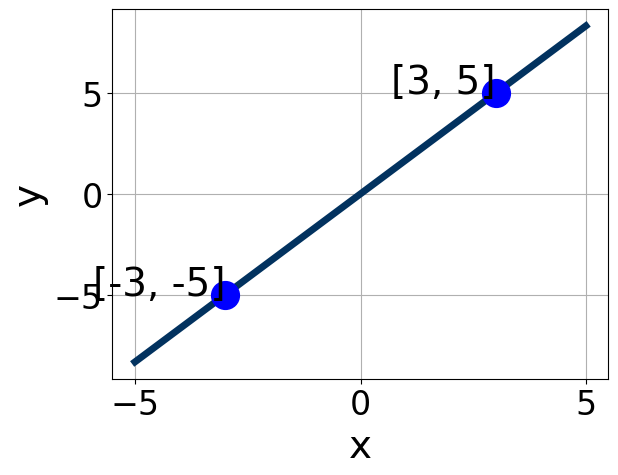
\includegraphics[width=0.5\textwidth]{../Figures/linearGraphToStandardCopyB.png}
\end{center}
\begin{enumerate}[label=\Alph*.]
\item \( A \in [-6, -2], \hspace{3mm} B \in [2, 3.6], \text{ and } \hspace{3mm} C \in [-2, 3] \)
\item \( A \in [-1.67, 2.33], \hspace{3mm} B \in [-1.5, -0.4], \text{ and } \hspace{3mm} C \in [-2, 3] \)
\item \( A \in [-1.67, 2.33], \hspace{3mm} B \in [0, 2.7], \text{ and } \hspace{3mm} C \in [-2, 3] \)
\item \( A \in [4, 7], \hspace{3mm} B \in [-3.9, -2.5], \text{ and } \hspace{3mm} C \in [-2, 3] \)
\item \( A \in [4, 7], \hspace{3mm} B \in [2, 3.6], \text{ and } \hspace{3mm} C \in [-2, 3] \)

\end{enumerate} }
\litem{
Solve the equation below. Then, choose the interval that contains the solution.\[ -8(-2x -18) = -19(-9x + 12) \]\begin{enumerate}[label=\Alph*.]
\item \( x \in [0.54, 0.65] \)
\item \( x \in [2.15, 2.72] \)
\item \( x \in [-0.7, -0.54] \)
\item \( x \in [0.23, 0.52] \)
\item \( \text{There are no real solutions.} \)

\end{enumerate} }
\litem{
First, find the equation of the line containing the two points below. Then, write the equation in the form $ y=mx+b $ and choose the intervals that contain $m$ and $b$.\[ (-8, 5) \text{ and } (6, -3) \]\begin{enumerate}[label=\Alph*.]
\item \( m \in [-1.48, 0.27] \hspace*{3mm} b \in [12.66, 13.75] \)
\item \( m \in [0.51, 0.74] \hspace*{3mm} b \in [-7.37, -5.63] \)
\item \( m \in [-1.48, 0.27] \hspace*{3mm} b \in [-0.63, 0.31] \)
\item \( m \in [-1.48, 0.27] \hspace*{3mm} b \in [0.36, 0.67] \)
\item \( m \in [-1.48, 0.27] \hspace*{3mm} b \in [-9.97, -8.7] \)

\end{enumerate} }
\litem{
Write the equation of the line in the graph below in Standard Form $Ax+By=C$. Then, choose the intervals that contain $A, B, \text{ and } C$.
\begin{center}
    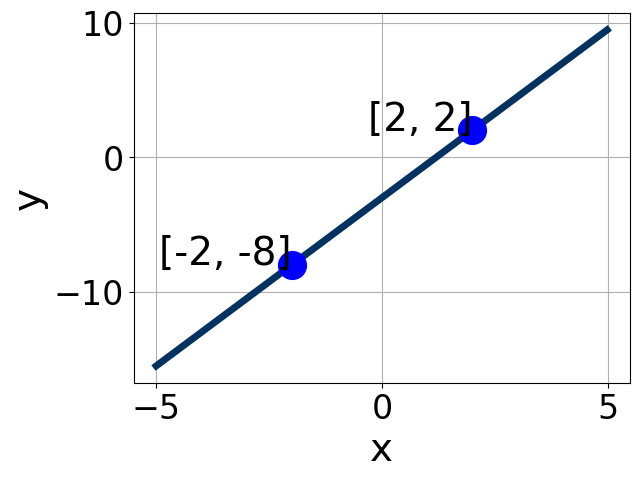
\includegraphics[width=0.5\textwidth]{../Figures/linearGraphToStandardB.png}
\end{center}
\begin{enumerate}[label=\Alph*.]
\item \( A \in [-2.6, 1.8], \hspace{3mm} B \in [-1.74, -0.89], \text{ and } \hspace{3mm} C \in [1.8, 4] \)
\item \( A \in [2.5, 8.3], \hspace{3mm} B \in [1.11, 2.52], \text{ and } \hspace{3mm} C \in [-7.9, -4.8] \)
\item \( A \in [2.5, 8.3], \hspace{3mm} B \in [-2.09, -1.79], \text{ and } \hspace{3mm} C \in [4.8, 8] \)
\item \( A \in [-5.1, -3.2], \hspace{3mm} B \in [1.11, 2.52], \text{ and } \hspace{3mm} C \in [-7.9, -4.8] \)
\item \( A \in [-2.6, 1.8], \hspace{3mm} B \in [-0.04, 1.53], \text{ and } \hspace{3mm} C \in [-5.2, -2.6] \)

\end{enumerate} }
\litem{
Solve the equation below. Then, choose the interval that contains the solution.\[ -14(-15x -6) = -3(18x -12) \]\begin{enumerate}[label=\Alph*.]
\item \( x \in [0.31, 0.74] \)
\item \( x \in [-1.04, -0.76] \)
\item \( x \in [-0.27, -0.14] \)
\item \( x \in [-0.53, -0.33] \)
\item \( \text{There are no real solutions.} \)

\end{enumerate} }
\litem{
Solve the linear equation below. Then, choose the interval that contains the solution.\[ \frac{-3x + 8}{2} - \frac{-8x -7}{3} = \frac{9x + 6}{4} \]\begin{enumerate}[label=\Alph*.]
\item \( x \in [7.9, 9] \)
\item \( x \in [4.4, 5.4] \)
\item \( x \in [0.6, 2] \)
\item \( x \in [0, 0.4] \)
\item \( \text{There are no real solutions.} \)

\end{enumerate} }
\litem{
Find the equation of the line described below. Write the linear equation in the form $ y=mx+b $ and choose the intervals that contain $m$ and $b$.\[ \text{Parallel to } 6 x + 7 y = 12 \text{ and passing through the point } (10, -4). \]\begin{enumerate}[label=\Alph*.]
\item \( m \in [0.16, 1.19] \hspace*{3mm} b \in [-13.13, -12.4] \)
\item \( m \in [-1.07, -0.35] \hspace*{3mm} b \in [2.89, 5.54] \)
\item \( m \in [-1.07, -0.35] \hspace*{3mm} b \in [-6.03, -3.72] \)
\item \( m \in [-1.26, -1.1] \hspace*{3mm} b \in [2.89, 5.54] \)
\item \( m \in [-1.07, -0.35] \hspace*{3mm} b \in [-14.4, -13.93] \)

\end{enumerate} }
\litem{
Solve the linear equation below. Then, choose the interval that contains the solution.\[ \frac{4x + 9}{3} - \frac{4x -4}{7} = \frac{9x + 6}{8} \]\begin{enumerate}[label=\Alph*.]
\item \( x \in [4.62, 5.62] \)
\item \( x \in [18.28, 21.28] \)
\item \( x \in [-1.69, 2.31] \)
\item \( x \in [4.77, 8.77] \)
\item \( \text{There are no real solutions.} \)

\end{enumerate} }
\litem{
Find the equation of the line described below. Write the linear equation in the form $ y=mx+b $ and choose the intervals that contain $m$ and $b$.\[ \text{Perpendicular to } 5 x - 7 y = 7 \text{ and passing through the point } (6, 10). \]\begin{enumerate}[label=\Alph*.]
\item \( m \in [-2.2, -1.21] \hspace*{3mm} b \in [3, 8] \)
\item \( m \in [-1.13, -0.18] \hspace*{3mm} b \in [18.4, 19.4] \)
\item \( m \in [1.05, 1.97] \hspace*{3mm} b \in [0.6, 2.6] \)
\item \( m \in [-2.2, -1.21] \hspace*{3mm} b \in [18.4, 19.4] \)
\item \( m \in [-2.2, -1.21] \hspace*{3mm} b \in [-21.4, -16.4] \)

\end{enumerate} }
\end{enumerate}

\end{document}